\documentclass[aspectratio=169,10pt]{beamer}

\usetheme{Madrid}
\usecolortheme{dolphin}
\setbeamertemplate{navigation symbols}{}
\setbeamertemplate{footline}[frame number]

\usepackage[utf8]{inputenc}
\usepackage[T1]{fontenc}
\usepackage[french]{babel}
\usepackage{lmodern}
\usepackage{graphicx}
\usepackage{booktabs}
\usepackage{array}
\usepackage{tabularx}
\usepackage{amsmath}
\usepackage{hyperref}
\usepackage{xcolor}
\usepackage{ragged2e}
\usepackage{tikz}
\usetikzlibrary{arrows.meta,positioning,shapes.geometric}

\definecolor{UniBlue}{RGB}{30,67,116}
\definecolor{SoftBlue}{RGB}{236,243,250}
\definecolor{DeepRed}{RGB}{166,38,38}
\definecolor{DarkGreen}{RGB}{28,112,77}
\definecolor{Gold}{RGB}{194,145,34}
\setbeamercolor{structure}{fg=UniBlue}
\setbeamercolor{frametitle}{fg=white,bg=UniBlue}
\setbeamercolor{title}{fg=UniBlue}
\setbeamercolor{block title}{fg=white,bg=UniBlue}
\setbeamercolor{block body}{bg=SoftBlue}
\setbeamerfont{frametitle}{series=\bfseries,size=\large}

\newcommand{\source}[1]{\vspace{0.15em}{\tiny\color{gray}Source : #1}}
\newcommand{\important}[1]{\textcolor{DeepRed}{\textbf{#1}}}
\newcommand{\ok}[1]{\textcolor{DarkGreen}{\textbf{#1}}}
\newcolumntype{Y}{>{\RaggedRight\arraybackslash}X}

\graphicspath{{../../presentation_assets/beamer_assets/}{../../figures/}{../../presentation_assets/chimerax/outputs/}}

\title[Interprétation de variants par structure 3D et MD]{Amélioration de l'interprétation de variants génétique par l'intégration de structure 3D de protéine et de données de dynamique moléculaire}
\subtitle{Comparaison de l'hémoglobine normale (WT) et de l'hémoglobine S (HbS)}
\author[Makwiza et al.]{Makwiza Mbala Judicael \and Matendo Kalaki Donat \and Mwanza Parousia Ketsia \\ Mfushi Kapalay Stephen \and Luayi Kangombo Jonas}
\institute{Université de Kinshasa -- Faculté des Sciences et Technologies\\Département de Mathématiques, Statistique et Informatique}
\date{Travail Pratique de Bioinformatique -- Master 2\\[0.25em]Titulaire : Professeur Christian D. BOPE \quad | \quad Doctorant : Keph Makoy}

\begin{document}

% 1 -----------------------------------------------------------------
\begin{frame}[plain]
\begin{columns}[c,totalwidth=\textwidth]
\begin{column}{0.15\textwidth}
\centering

\includegraphics[width=0.83\linewidth,keepaspectratio]{unikin_logo.png}
\end{column}
\begin{column}{0.82\textwidth}
\centering
{\scriptsize UNIVERSITÉ DE KINSHASA -- FACULTÉ DES SCIENCES ET TECHNOLOGIES}\par
\vspace{0.5em}
{\color{UniBlue}\bfseries\fontsize{15}{18}\selectfont
Amélioration de l'interprétation de variants génétique par l'intégration de structure 3D de protéine et de données de dynamique moléculaire\par}
\vspace{0.45em}
{\small\bfseries Comparaison de l'hémoglobine normale (WT) et de l'hémoglobine S (HbS)}
\end{column}
\end{columns}

\vspace{0.6em}
\begin{columns}[T,totalwidth=0.94\textwidth]
\begin{column}{0.56\textwidth}
\begin{block}{Membres du groupe}
\footnotesize
\begin{tabular}{@{}l@{}}
Makwiza Mbala Judicael\\
Matendo Kalaki Donat\\
Mwanza Parousia Ketsia\\
Mfushi Kapalay Stephen\\
Luayi Kangombo Jonas
\end{tabular}
\end{block}
\end{column}
\begin{column}{0.38\textwidth}
\begin{block}{Encadrement}
\footnotesize
\textbf{Titulaire :} Professeur Christian D. BOPE\\[0.35em]
\textbf{Doctorant :} Keph Makoy\\[0.35em]
\textbf{Promotion :} Master 2
\end{block}
\end{column}
\end{columns}
\vfill
\begin{center}
{\small\textbf{Travail Pratique de Bioinformatique} -- Année académique 2025--2026}
\end{center}
\end{frame}

% 2 -----------------------------------------------------------------
\begin{frame}{Introduction : hémoglobine, HbS et drépanocytose}
\begin{columns}[T,totalwidth=\textwidth]
\begin{column}{0.48\textwidth}
\begin{block}{Contexte}
\footnotesize
L'hémoglobine adulte est une protéine tétramérique \(\alpha_2\beta_2\) contenant quatre groupes hème. Le gène \textbf{HBB} code la chaîne \(\beta\). Le variant \textbf{c.20A>T} produit l'hémoglobine S (HbS), décrite classiquement comme \textbf{\(\beta\)Glu6Val} dans la chaîne mature.
\end{block}
\begin{block}{Pourquoi cette mutation est importante ?}
\footnotesize
Le remplacement d'un glutamate chargé par une valine hydrophobe modifie localement la surface de la chaîne \(\beta\). En condition désoxygénée, ce changement favorise des contacts entre molécules HbS et participe à leur polymérisation, mécanisme central de la drépanocytose.
\end{block}
\end{column}
\begin{column}{0.49\textwidth}
\centering

\includegraphics[width=0.95\linewidth,height=0.36\textheight,keepaspectratio]{WT_global.png}
\vspace{0.15em}

{\scriptsize Architecture de l'hémoglobine : 4 chaînes et 4 hèmes.}
\vspace{0.3em}

\begin{columns}[T,totalwidth=\linewidth]
\begin{column}{0.49\linewidth}\centering

\includegraphics[width=\linewidth,height=0.22\textheight,keepaspectratio]{WT_GLU6_closeup.png}
{\tiny WT : GLU6}
\end{column}
\begin{column}{0.49\linewidth}\centering

\includegraphics[width=\linewidth,height=0.22\textheight,keepaspectratio]{HbS_VAL6_closeup.png}
{\tiny HbS : VAL6}
\end{column}
\end{columns}
\end{column}
\end{columns}
\vspace{0.2em}
{\scriptsize\textbf{Dépôt du projet :} \href{https://github.com/JudicaelMAKWIZA/HBB_MD_Interpretation}{\textcolor{UniBlue}{\texttt{github.com/JudicaelMAKWIZA/HBB\_MD\_Interpretation}}}. Les détails du protocole, scripts et résultats reproductibles sont documentés dans le \texttt{README.md}.}
\source{ClinVar : HBB c.20A>T (p.Glu7Val) / HbS / rs334 ; RCSB PDB 2DN2 et 2HBS.}
\end{frame}

% 3 -----------------------------------------------------------------
\begin{frame}{Problématique, hypothèse et objectifs}
\begin{block}{Problématique}
\small
Dans quelle mesure l'intégration de l'annotation clinique, de structures 3D expérimentales et de métriques issues d'une dynamique moléculaire permet-elle de mieux interpréter l'impact structural du variant HBB \(\beta\)Glu6Val ?
\end{block}

\begin{columns}[T,totalwidth=\textwidth]
\begin{column}{0.47\textwidth}
\begin{block}{Hypothèse}
\footnotesize
La substitution Glu \(\rightarrow\) Val peut produire des différences mesurables de dynamique et de compacité. Sur un tétramère isolé, ces différences devraient rester modestes si le mécanisme pathogène dépend surtout des interactions \textbf{intermoléculaires}.
\end{block}
\end{column}
\begin{column}{0.50\textwidth}
\begin{block}{Objectifs}
\footnotesize
\begin{enumerate}
  \item Documenter le variant HBB étudié et son contexte clinique.
  \item Comparer les structures 3D WT et HbS.
  \item Préparer et simuler les deux modèles moléculaires dans les mêmes conditions.
  \item Quantifier stabilité, flexibilité et compacité par RMSD, RMSF et rayon de giration.
  \item Relier ces observations à l'interprétation biologique du variant.
\end{enumerate}
\end{block}
\end{column}
\end{columns}
\end{frame}

% 4 -----------------------------------------------------------------
\begin{frame}{Méthodes : pipeline d'analyse}
\small
\begin{center}
\begin{tikzpicture}[scale=0.94,transform shape,
node distance=0.30cm,
box/.style={draw=UniBlue,rounded corners=2pt,fill=SoftBlue,minimum height=0.82cm,text width=2.15cm,align=center,font=\scriptsize\bfseries},
arr/.style={-{Latex[length=2.3mm]},thick,draw=UniBlue}
]
\node[box] (v) {1. Variant\\ClinVar};
\node[box,right=of v] (p) {2. Structures\\2DN2 / 2HBS};
\node[box,right=of p] (prep) {3. Préparation\\GROMACS};
\node[box,right=of prep] (eq) {4. Équilibration\\EM, NVT, NPT};
\node[box,right=of eq] (md) {5. Production\\1 ns};
\node[box,right=of md] (ana) {6. Analyses\\RMSD, RMSF, Rg};
\draw[arr] (v)--(p); \draw[arr] (p)--(prep); \draw[arr] (prep)--(eq); \draw[arr] (eq)--(md); \draw[arr] (md)--(ana);
\end{tikzpicture}
\end{center}

\vspace{0.5em}
\begin{columns}[T,totalwidth=\textwidth]
\begin{column}{0.48\textwidth}
\begin{block}{De la donnée biologique au modèle 3D}
\footnotesize
\textbf{Variant :} identification de HBB c.20A>T et de son effet Glu6Val.\\
\textbf{Structures :} sélection de l'hémoglobine WT (2DN2) et HbS (2HBS), conservation des chaînes A--D et des hèmes.\\
\textbf{Préparation :} protonation contrôlée, topologie des hèmes, boîte commune, solvatation et NaCl 0,15 M.
\end{block}
\end{column}
\begin{column}{0.49\textwidth}
\begin{block}{De la simulation à l'interprétation}
\footnotesize
\textbf{Équilibration :} éliminer les contacts défavorables puis stabiliser température et pression avant l'analyse.\\
\textbf{Production :} trajectoire pilote de 1 ns pour chaque modèle.\\
\textbf{Analyses :} RMSD (stabilité globale), RMSF (mobilité par résidu), Rg (compacité) et visualisation ChimeraX de Glu6/Val6.
\end{block}
\end{column}
\end{columns}
\source{GROMACS 2023.3 ; UCSF ChimeraX ; scripts et fichiers MDP disponibles dans le dépôt GitHub.}
\end{frame}

% 5 -----------------------------------------------------------------
\begin{frame}{Préparation et validation}
\small
\begin{block}{Que fait cette étape ?}
\footnotesize
Elle transforme les structures cristallographiques en \textbf{modèles moléculaires comparables et simulables} : même volume périodique, même concentration saline, hèmes conservés et topologie cohérente. WT et HbS sont ici deux \textbf{modèles moléculaires} représentant les deux formes de l'hémoglobine.
\end{block}

\begin{columns}[T,totalwidth=\textwidth]
\begin{column}{0.51\textwidth}
\begin{block}{Paramètres de préparation}
\footnotesize
\begin{itemize}
  \item GROMACS 2023.3 ; champ de force \textbf{GROMOS54A7\_hbb} ; eau SPC.
  \item Boîte dodécaédrique commune : \textbf{682,654 nm\(^3\)}.
  \item NaCl \textbf{0,15 M} et neutralisation des charges.
  \item Profil d'histidines commun ; quatre liaisons proximales His--Fe prises en compte.
\end{itemize}
\end{block}
\end{column}
\begin{column}{0.46\textwidth}
\begin{block}{Contrôles de qualité}
\footnotesize
\begin{itemize}
  \item 4 hèmes présents pour WT et HbS.
  \item Aucun angle G96 manquant après correctif local documenté.
  \item Aucun \textit{LINCS warning} pendant l'équilibration et la production.
  \item Uniquement l'avertissement GROMOS connu accepté dans \texttt{grompp}.
\end{itemize}
\end{block}
\end{column}
\end{columns}
\vspace{0.05em}
\centering
\scriptsize
\begin{tabular}{lccc}
\toprule
Modèle & Atomes après ions & Eaux & Ions ajoutés \\
\midrule
WT & 65 571 & 19 879 & 68 Na\(^+\), 62 Cl\(^-\) \\
HbS & 65 415 & 19 829 & 66 Na\(^+\), 62 Cl\(^-\) \\
\bottomrule
\end{tabular}
\end{frame}

% 6 -----------------------------------------------------------------
\begin{frame}[shrink=1]{Équilibration et stabilité thermodynamique}
\small
\begin{block}{Pourquoi équilibrer avant la production ?}
\footnotesize
Après la minimisation, le modèle doit s'adapter progressivement à son environnement aqueux. Le NVT stabilise la \textbf{température} à 300 K ; le NPT ajuste ensuite la \textbf{pression et la densité}. Les contraintes de position sont retirées avant la production afin d'observer la dynamique propre de la protéine.
\end{block}

\begin{columns}[T,totalwidth=\textwidth]
\begin{column}{0.46\textwidth}
\begin{block}{Protocole}
\footnotesize
\begin{tabular}{p{0.58\linewidth}p{0.29\linewidth}}
\toprule
Étape & Durée / critère \\
\midrule
Minimisation & Fmax $<$ 1000 \\
NVT, contraintes & 100 ps \\
NPT, contraintes & 300 ps \\
NPT libre & 200 ps \\
Production & 1 ns \\
\bottomrule
\end{tabular}
\end{block}
\begin{block}{Minimisation}
\scriptsize
WT : 523 étapes, Fmax = 959,85 kJ mol\(^{-1}\) nm\(^{-1}\).\\
HbS : 552 étapes, Fmax = 943,06 kJ mol\(^{-1}\) nm\(^{-1}\).
\end{block}
\end{column}
\begin{column}{0.51\textwidth}
\begin{block}{Production 1 ns : moyenne $\pm$ écart-type}
\footnotesize
\begin{tabular}{lcc}
\toprule
Métrique & WT & HbS \\
\midrule
Température (K) & 299,94 $\pm$ 1,26 & 299,88 $\pm$ 1,31 \\
Pression (bar) & 0,32 $\pm$ 106,81 & -0,01 $\pm$ 102,22 \\
Densité (kg/m\(^3\)) & 1017,59 $\pm$ 1,90 & 1016,93 $\pm$ 1,87 \\
\bottomrule
\end{tabular}
\end{block}
\begin{block}{Interprétation}
\footnotesize
Les températures et densités sont stables et quasi identiques entre WT et HbS. La pression instantanée fluctue fortement, comportement attendu à l'échelle atomistique ; sa moyenne reste proche de la valeur cible.
\end{block}
\end{column}
\end{columns}
\end{frame}

% 7 -----------------------------------------------------------------
\begin{frame}{Résultats globaux : stabilité et compacité}
\begin{columns}[T,totalwidth=\textwidth]
\begin{column}{0.50\textwidth}
\centering
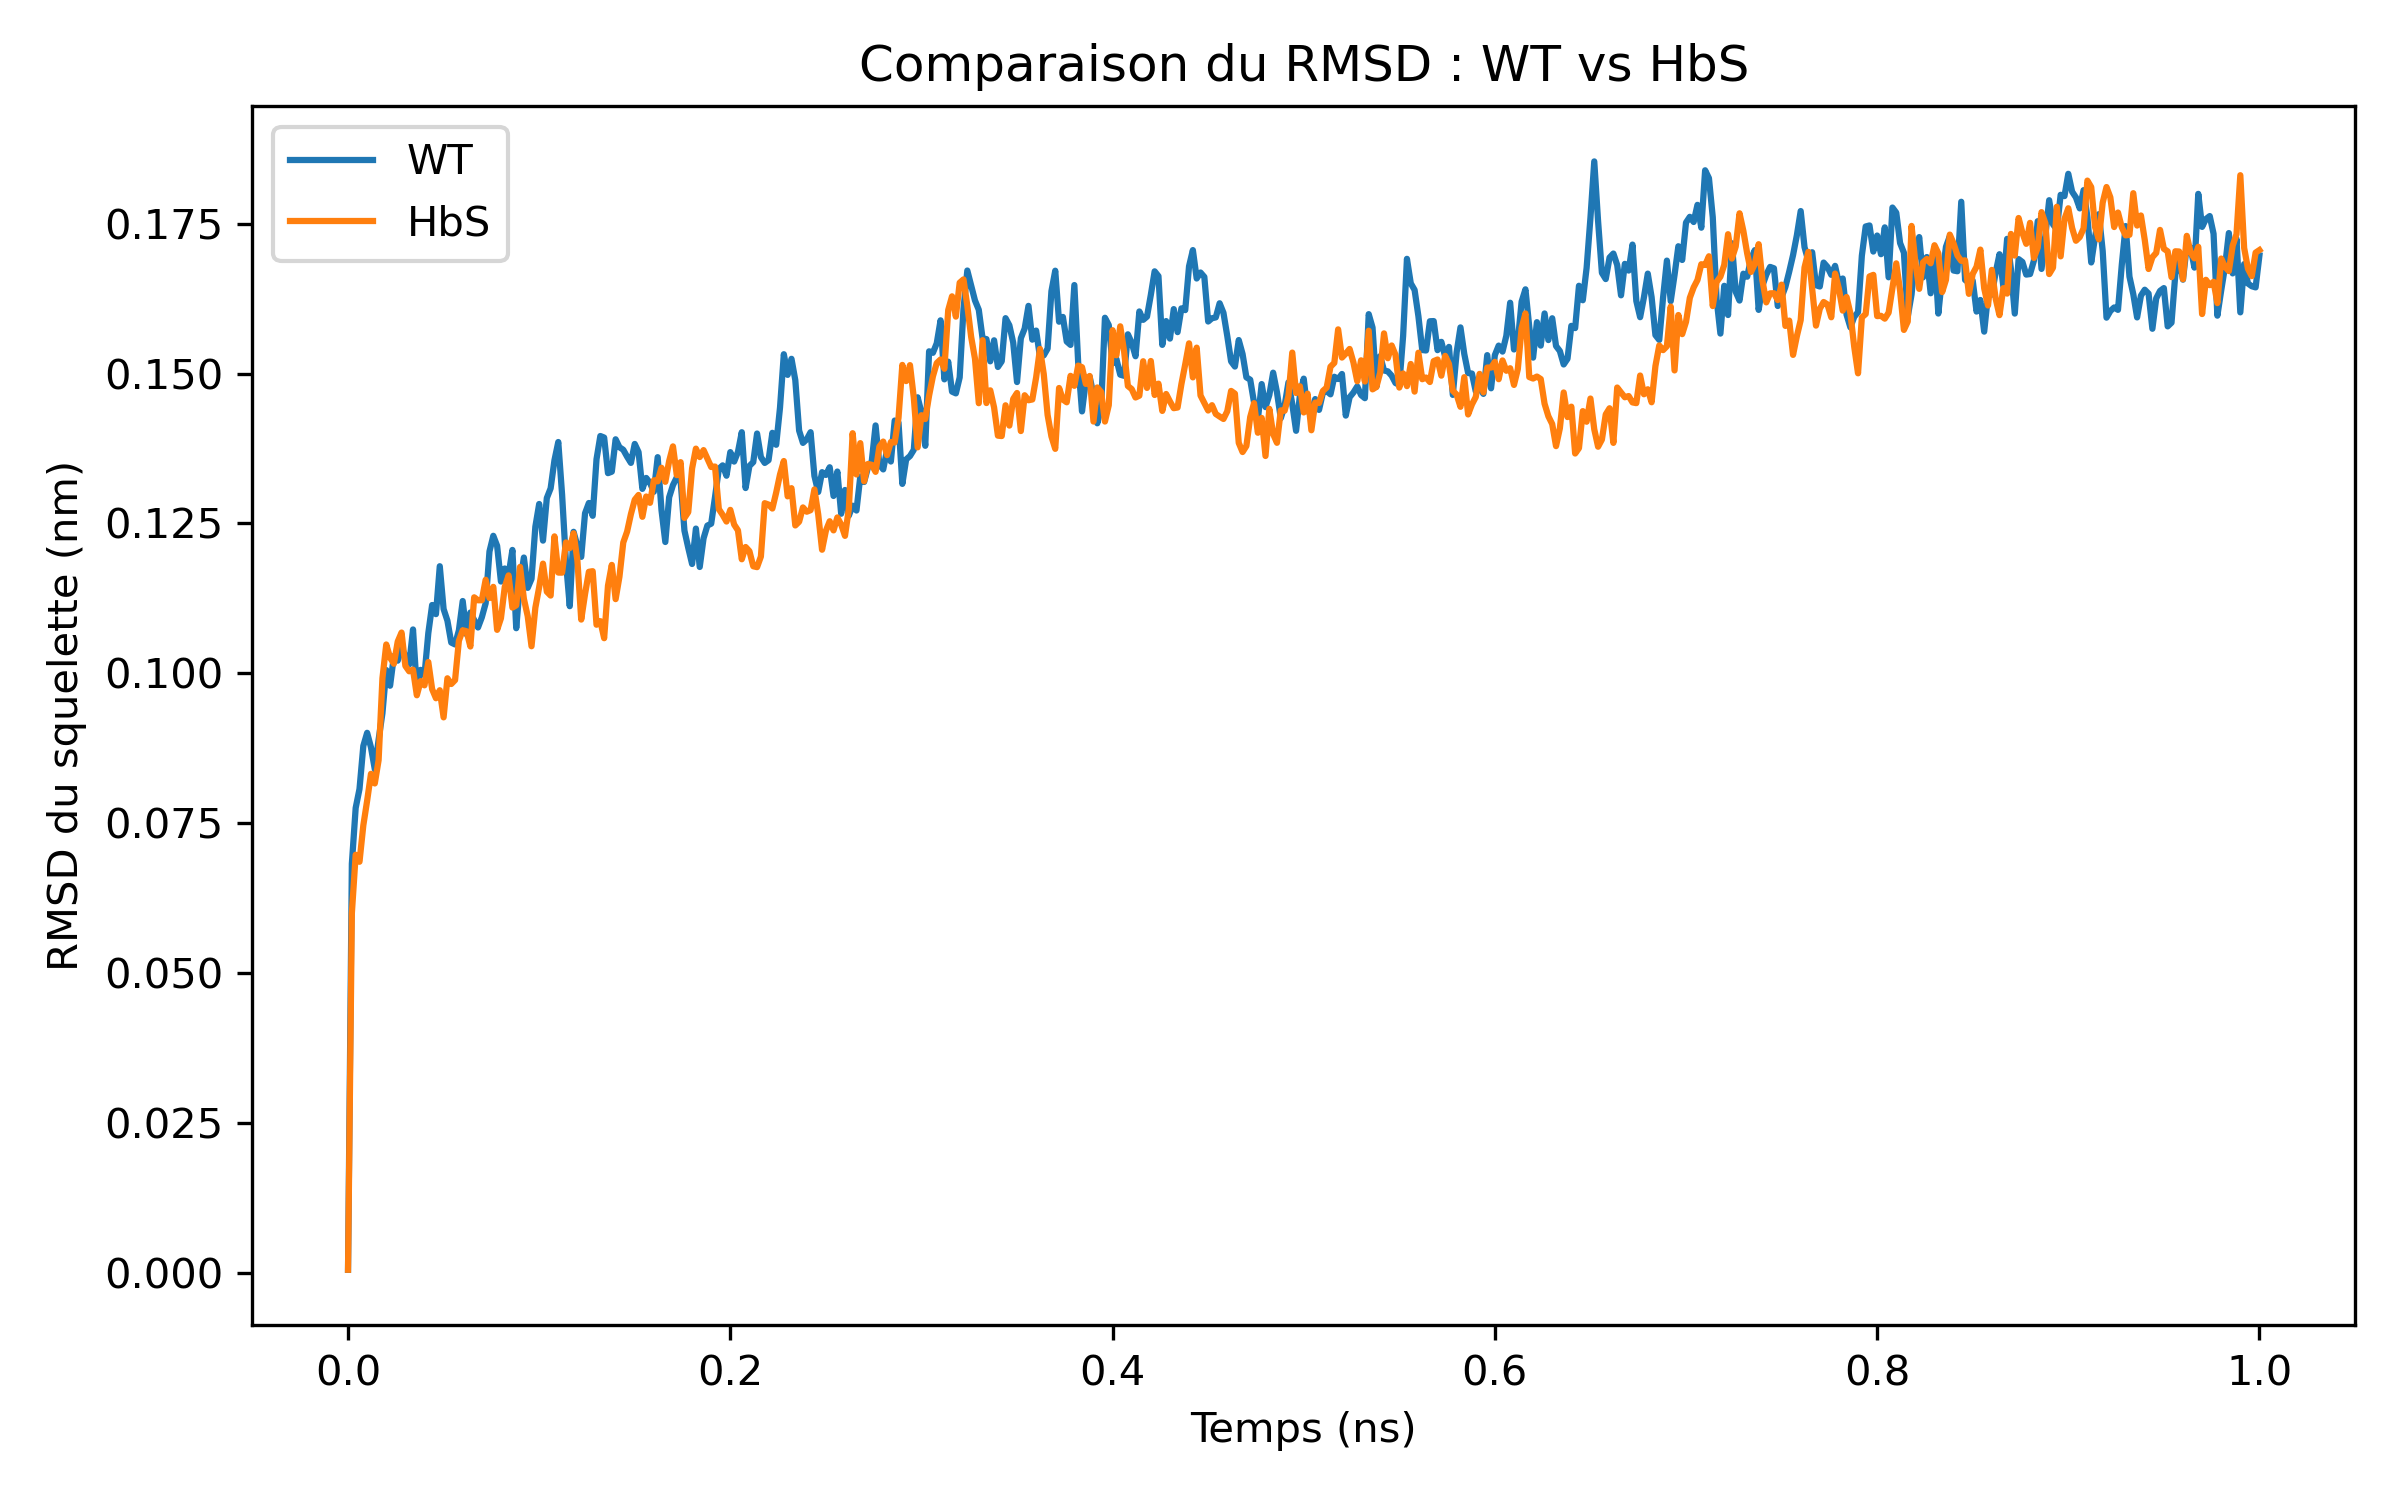
\includegraphics[width=\linewidth,height=0.47\textheight,keepaspectratio]{rmsd.png}
{\scriptsize RMSD du squelette : évolution de l'écart à la structure de référence.}
\end{column}
\begin{column}{0.50\textwidth}
\centering
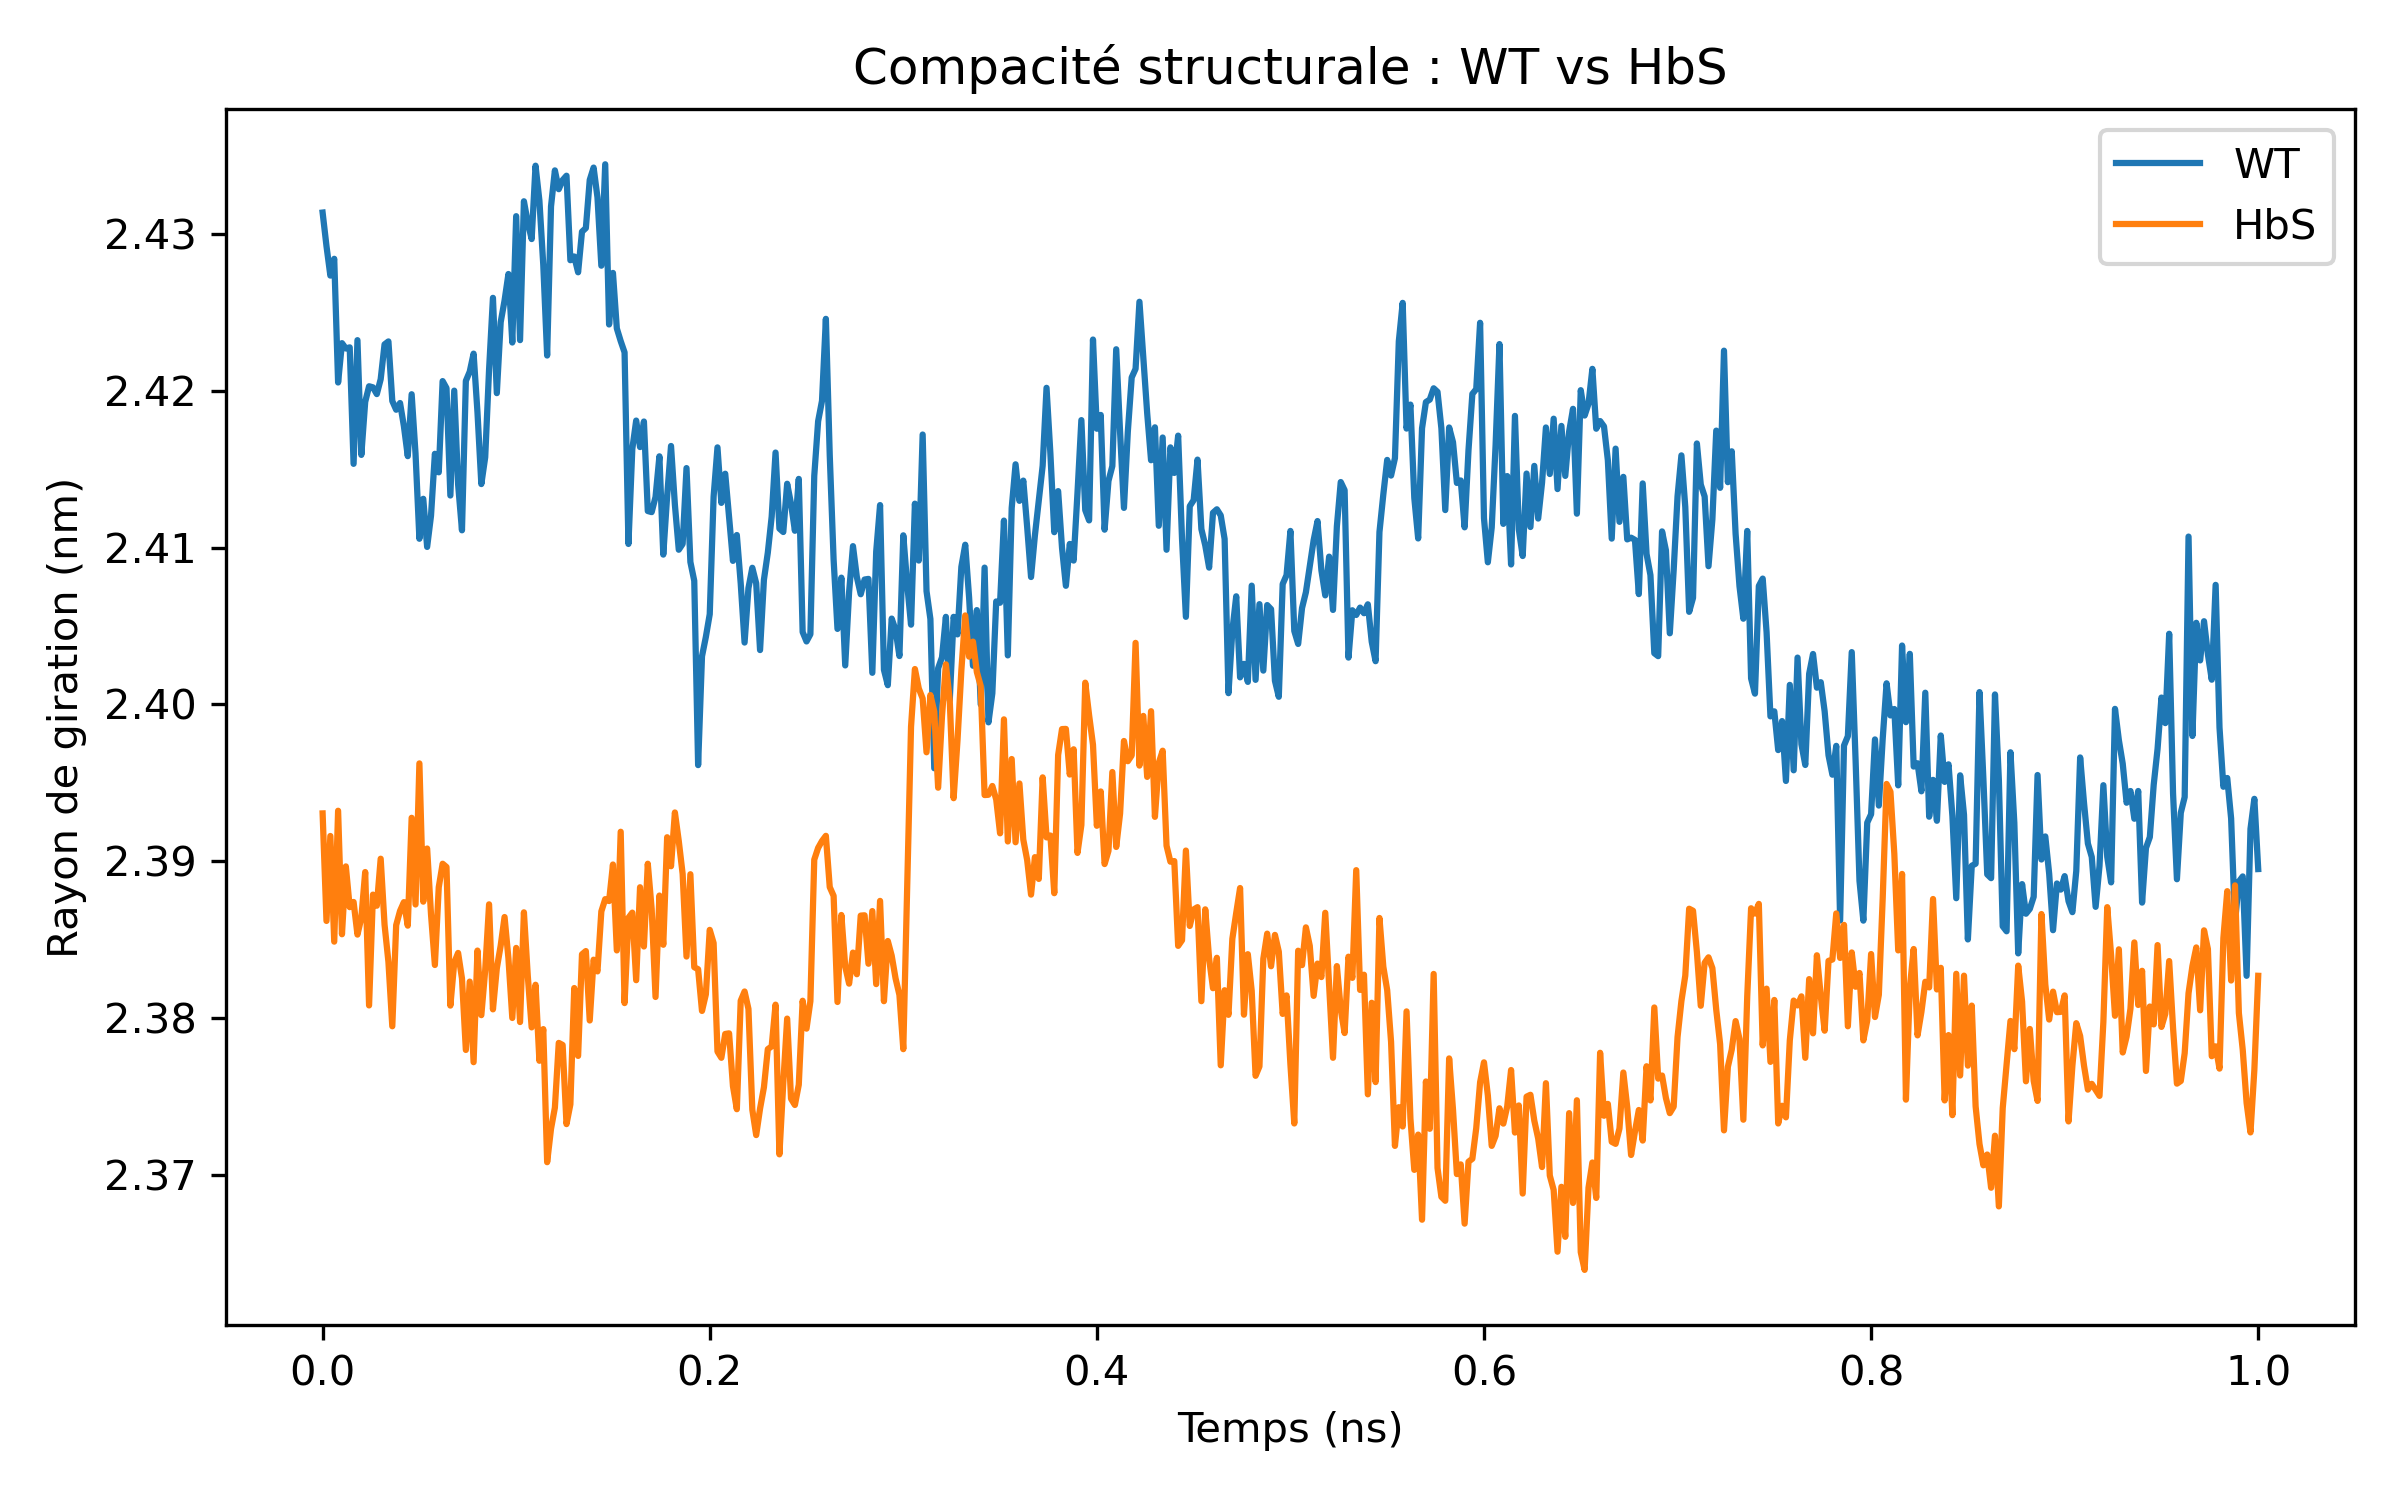
\includegraphics[width=\linewidth,height=0.47\textheight,keepaspectratio]{rg.png}
{\scriptsize Rayon de giration : mesure de la compacité du tétramère.}
\end{column}
\end{columns}

\vspace{0.25em}
\scriptsize
\begin{tabularx}{\textwidth}{lcccY}
\toprule
Métrique & WT & HbS & $\Delta$ HbS-WT & Ce que cela signifie \\
\midrule
RMSD moyen (0,2--1 ns) & 0,1581 $\pm$ 0,0122 & 0,1533 $\pm$ 0,0140 & -0,0048 nm & Les deux structures restent très proches en stabilité globale. \\
Rg moyen (0,2--1 ns) & 2,4059 $\pm$ 0,0096 & 2,3821 $\pm$ 0,0083 & -0,0238 nm & HbS est légèrement plus compacte, sans changement majeur. \\
\bottomrule
\end{tabularx}
\vspace{0.15em}
\begin{center}
\footnotesize\important{Résultat clé :} aucune déstabilisation globale importante de HbS n'est observée sur cette trajectoire pilote de 1 ns.
\end{center}
\end{frame}

% 8 -----------------------------------------------------------------
\begin{frame}{Résultats locaux : flexibilité et mutation \texorpdfstring{$\beta$}{β}6}
\begin{columns}[T,totalwidth=\textwidth]
\begin{column}{0.47\textwidth}
\centering
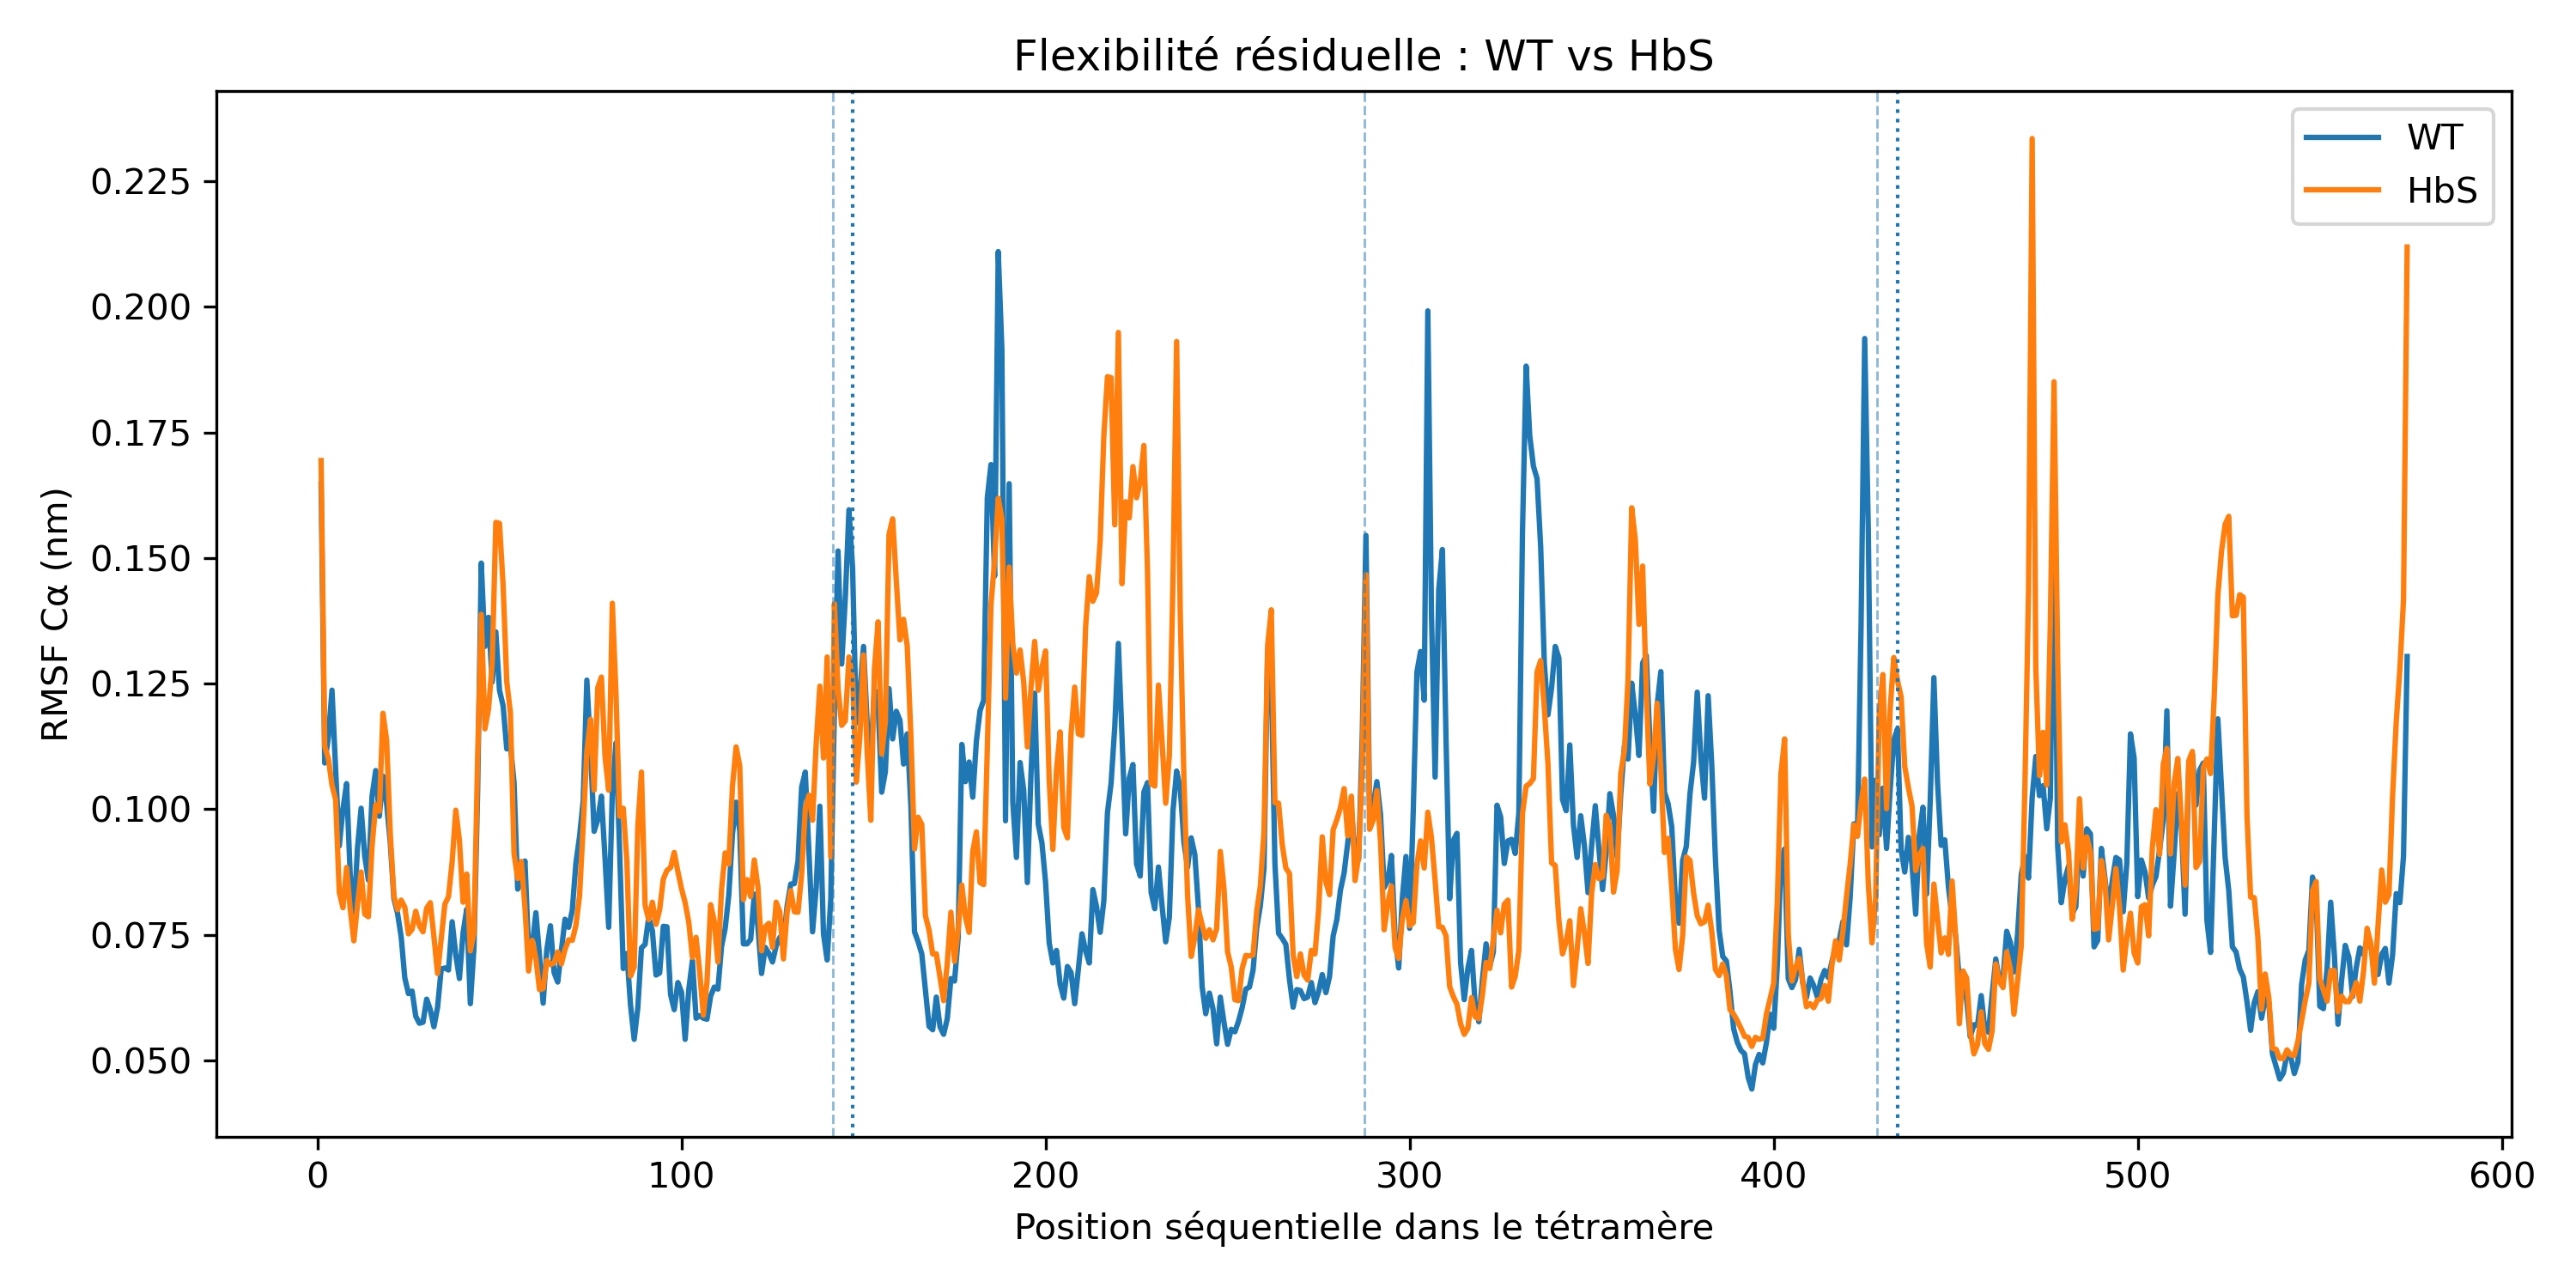
\includegraphics[width=\linewidth,height=0.48\textheight,keepaspectratio]{rmsf.png}
\vspace{0.2em}

\scriptsize
\begin{tabular}{lcc}
\toprule
RMSF (nm) & WT & HbS \\
\midrule
C\(\alpha\) moyen & 0,0882 & 0,0932 \\
\(\beta\)6 moyen & 0,1320 & 0,1258 \\
Voisinage \(\beta\)6 $\pm$5 & 0,1144 & 0,1164 \\
\bottomrule
\end{tabular}
\end{column}
\begin{column}{0.50\textwidth}
\begin{columns}[T,totalwidth=\linewidth]
\begin{column}{0.49\linewidth}\centering

\includegraphics[width=\linewidth,height=0.22\textheight,keepaspectratio]{WT_GLU6_closeup.png}
{\tiny WT : glutamate en position \(\beta\)6}
\end{column}
\begin{column}{0.49\linewidth}\centering

\includegraphics[width=\linewidth,height=0.22\textheight,keepaspectratio]{HbS_VAL6_closeup.png}
{\tiny HbS : valine en position \(\beta\)6}
\end{column}
\end{columns}
\vspace{0.25em}
\centering

\includegraphics[width=0.92\linewidth,height=0.24\textheight,keepaspectratio]{WT_vs_HbS_overlay.png}
\vspace{0.15em}
\begin{block}{Lecture}
\footnotesize
HbS présente un RMSF global légèrement supérieur, mais la position \(\beta\)6 ne devient pas nettement plus mobile. La substitution est donc structurale et chimique sans produire, ici, une forte instabilité locale mesurable.
\end{block}
\end{column}
\end{columns}
\end{frame}

% 9 -----------------------------------------------------------------
\begin{frame}{Conclusion, limites et remerciements}
\begin{columns}[T,totalwidth=\textwidth]
\begin{column}{0.61\textwidth}
\begin{block}{Conclusion}
\footnotesize
L'intégration de l'annotation clinique, de la visualisation 3D et de la dynamique moléculaire a permis d'interpréter le variant HBB \(\beta\)Glu6Val à plusieurs niveaux. Sur 1 ns, WT et HbS restent globalement stables et proches ; les différences observées concernent surtout de faibles variations de flexibilité et de compacité.
\end{block}
\begin{block}{Interprétation biologique}
\footnotesize
Ces résultats sont compatibles avec un mécanisme pathogène principalement \important{intermoléculaire} : la valine hydrophobe en \(\beta\)6 favorise les contacts entre molécules HbS et leur polymérisation plutôt qu'une simple déstabilisation du tétramère isolé.
\end{block}
\end{column}
\begin{column}{0.36\textwidth}
\begin{block}{Limites}
\scriptsize
\begin{itemize}
  \item Production courte : 1 ns par modèle.
  \item Structures WT et HbS issues de cristaux différents.
  \item Tétramère isolé : polymérisation de fibres non simulée.
  \item Résultats exploratoires, pas une estimation de \(\Delta G\).
\end{itemize}
\end{block}
\begin{block}{Remerciements}
\scriptsize
Nous remercions le \textbf{Professeur Christian D. BOPE}, titulaire du cours, pour l'enseignement et l'encadrement, ainsi que le \textbf{Doctorant Keph Makoy} pour son orientation scientifique et son accompagnement dans la réalisation de ce travail.
\end{block}
\end{column}
\end{columns}
\end{frame}

% 10 ----------------------------------------------------------------
\begin{frame}[shrink=2]{Références et reproductibilité}
\small
\begin{columns}[T,totalwidth=\textwidth]
\begin{column}{0.62\textwidth}
\begin{block}{Références principales}
\tiny
\begin{itemize}
  \item BOPE, C. D. \textit{Programmation et algorithmes pour la bioinformatique - Notes de cours détaillées}. Université de Kinshasa, 2025--2026.
  \item NCBI ClinVar. \textit{NM\_000518.5(HBB):c.20A>T (p.Glu7Val), HbS, rs334}.
  \item RCSB PDB. \textbf{2DN2} : human deoxyhemoglobin, 1,25 \AA ; \textbf{2HBS} : deoxyhemoglobin S, 2,05 \AA.
  \item Harrington, D. J.; Adachi, K.; Royer, W. E. \textit{The high resolution crystal structure of deoxyhemoglobin S}. J. Mol. Biol. 272, 398--407, 1997.
  \item Abraham, M. J. et al. \textit{GROMACS: High performance molecular simulations through multi-level parallelism}. SoftwareX 1--2, 19--25, 2015 ; documentation GROMACS 2023.3.
  \item Pettersen, E. F. et al. \textit{UCSF ChimeraX: Structure visualization for researchers, educators, and developers}. Protein Sci. 30, 70--82, 2021.
\end{itemize}
\end{block}
\end{column}
\begin{column}{0.35\textwidth}
\begin{block}{Dépôt reproductible}
\footnotesize
\href{https://github.com/JudicaelMAKWIZA/HBB_MD_Interpretation}{\textcolor{UniBlue}{\textbf{Ouvrir le dépôt GitHub}}}\\[0.45em]
\scriptsize\url{https://github.com/JudicaelMAKWIZA/HBB_MD_Interpretation}
\vspace{0.45em}

Le \texttt{README.md} contient les détails impossibles à développer en 10 diapositives : structures, paramètres GROMACS, étapes de validation, métriques, figures, limites et commandes de reproduction.
\end{block}
\begin{block}{Contenu disponible}
\scriptsize
\begin{itemize}
  \item scripts Python/Bash ;
  \item fichiers \texttt{.mdp} ;
  \item structures PDB préparées ;
  \item résultats numériques ;
  \item figures RMSD/RMSF/Rg ;
  \item visualisations ChimeraX ;
  \item source Beamer et PDF.
\end{itemize}
\end{block}
\end{column}
\end{columns}
\end{frame}

\end{document}
